\documentclass{ieeeaccess}
\usepackage{cite}
\usepackage{amsmath,amssymb,amsfonts}
\usepackage{graphicx}
\usepackage{textcomp}
\usepackage{hyperref}
\usepackage{tikz}
\usetikzlibrary{shapes.arrows,positioning}

\begin{document}
\doi{-}

\title{Generalization of Deep Learning-Based Waste Detection Across Riverine Environments: A Systematic Review}
\author{\uppercase{Yush Pokharel}\authorrefmark{1}}
\address[1]{Affiliation To Be Confirmed}
\corresp{Corresponding author: TBD (e-mail: TBD).}

\begin{keywords}
Deep Learning, Waste Detection, River Pollution, Generalization, Transfer Learning, UAV, Remote Sensing, Systematic Review
\end{keywords}

% NOTE: abstract.tex wraps its own abstract environment; input directly (before maketitle per IEEE Access convention).
\begin{abstract}
Rivers carry a large share of plastic pollution to the oceans, yet automated waste detection is rarely tested beyond its training environment. This review synthesizes 50 studies (2019--2025) on deep-learning and computer-vision waste detection across riverine environments, asking how well models generalize across rivers, regions, sensors, and conditions. Collection was seed-anchored and transparently reported without formal systematic-review protocol claims; each study was extracted into a uniform schema and graded on a four-level generalization scale. Transfer within bounds is well supported: proximate rivers, similar sites, and matched spectra transfer reliably, while sediment shifts, land-to-water jumps, and narrow-channel pixel mixing cause sharp failures. YOLO-family detectors dominate field deployment, segmentation wins area estimation, instance-level and transformer studies are nearly absent, and open datasets plus self-supervised and adaptive methods are easing annotation scarcity. Crucially, detection scores overstate counting reliability, and no riverine underwater study exists. The review delivers a transferability map and a gap inventory oriented to resource-limited settings where cross-environment generalization matters most.
\end{abstract}


\maketitle

% Sections (\input-ready fragments, no preambles)
\section{Introduction}
\label{sec:introduction}

In Kathmandu Valley, the Bishnumati and Bagmati rivers carry the visible signature of rapid urbanization: floating plastics that threaten water sustainability where waste management cannot keep pace \cite{Pati2025}. The local scene scales globally, with on the order of a thousand rivers accounting for most riverine plastic emissions to the ocean \cite{Meijer2021}. Monitoring this flux is therefore a first-order environmental task, yet the dominant methods --- manual counting, net sampling, visual survey --- are slow, subjective, spatially sparse, and dangerous during the flood pulses that move the most litter \cite{Lieshout2020,Hurley2023}. Automated detectors already count substantially more items than human observers under identical conditions \cite{Lieshout2020}, which motivates a shift from episodic inspection to continuous observation (Fig.~\ref{fig:problem}).
% Problem diagram for the introduction (referenced as Fig.~\ref{fig:problem}).
\begin{figure}[!t]
\centering
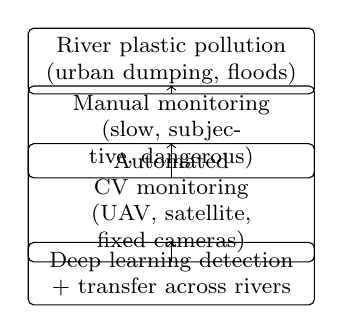
\begin{tikzpicture}[node distance=0.9cm, every node/.style={draw, rounded corners=2pt, text width=3.4cm, align=center, font=\footnotesize}]
\node (poll) {River plastic pollution\\(urban dumping, floods)};
\node (man) [below of=poll] {Manual monitoring\\(slow, subjective, dangerous)};
\node (auto) [below of=man] {Automated CV monitoring\\(UAV, satellite, fixed cameras)};
\node (dl) [below of=auto] {Deep learning detection\\+ transfer across rivers};
\draw[->] (poll) -- (man);
\draw[->] (man) -- (auto);
\draw[->] (auto) -- (dl);
\end{tikzpicture}
\caption{From river pollution evidence to automated monitoring: manual limits motivate continuous computer-vision observation, and deep learning must transfer across rivers to be useful.}
\label{fig:problem}
\end{figure}


Computer vision reframes rivers as scannable surfaces. Unmanned aerial vehicles deliver centimetre detail over reaches \cite{Maharjan2022,Jakovljevic2020}; satellites revisit whole basins at coarser grains \cite{SoleGomez2022,Mohsen2023}; bridge and bank cameras watch fixed cross-sections around the clock \cite{Lieshout2020,Reinhardt2024}; phones and citizen observers extend coverage where infrastructure is absent \cite{JiaFrontiers2023,Tharani2021}. Deep learning converts these pixels into detections, masks, and counts with rapidly maturing accuracy \cite{Jia2023}. The base study for this review exemplifies the state of the art: a controlled comparison of detection and segmentation under three training strategies with cross-river transfer tests on novel Nepali datasets \cite{Pati2025}.

What remains unanswered is generalization. Prior syntheses catalogue platforms \cite{Marye2025} and architectures \cite{Jia2023} but do not systematically ask whether a model trained on one river, sensor, or season works on another. This review fills that gap as the first generalization-centered synthesis of deep-learning waste detection across riverine environments. It contributes: (i) an evidence-graded corpus of 50 studies spanning UAV, satellite, fixed, handheld, surface-vehicle, and (by documented absence) underwater sensing; (ii) a four-level generalization grading applied uniformly, separating demonstrated transfer from claimed robustness; (iii) a replication record for the base study's findings across independent rivers and continents; and (iv) a gap inventory oriented to Nepal-like, resource-constrained settings where transfer learning matters most.

\section{Review Methodology}
\label{sec:methodology}

This review follows a structured methodology with transparent reporting of search, screening, and selection. It does not claim formal PRISMA protocol registration.

\subsection{Review Design and Seeds}
The collection is seed-anchored rather than database-exhaustive. Seed 1 (P001) is a comparative experimental study of UAV-based river waste detection that serves as the methodological blueprint (training strategies, UAV datasets, cross-river evaluation) \cite{Pati2025}. Seed 2 (P002) is a systematic review of remote sensing for river macroplastics that provides the state-of-the-art baseline and the backward-tracking corpus \cite{Marye2025}. Two further reviews (P003 on deep learning for macroplastic detection \cite{Jia2023}; P008's companion corpus) and the P004 early river-DL study \cite{Jakovljevic2020} extended the backward-tracking set.

\subsection{Sources Searched}
Backward citation tracking was performed over (i) the base-paper bibliography (\texttt{references.bib}), (ii) the WIREs review evidence tables, and (iii) three connected-paper export files ($\sim$122 titles, deduplicated against the collection). Targeted web retrieval acted as a proxy for Scopus, Web of Science, IEEE Xplore, MDPI, and ScienceDirect across keyword sweeps (river + UAV + deep learning; YOLO river waste; satellite river debris; pond/lake/canal detection; 2024--2026 architectures). No full database keyword pass and no Scholar/Scopus forward tracking were executed; both are recorded as deferred in the search log rather than silently omitted.

\subsection{Scope As Applied}
The working scope --- deep learning and computer vision for waste detection in rivers, ponds, and closely related freshwaters, 2015--2026, peer-reviewed journals and reputable conferences, global coverage with Nepal as guiding context --- describes the corpus as collected rather than gating it: all 50 included studies fall in 2019--2025 and meet the criteria as applied. Preprints and theses were held out regardless of relevance. One low-index venue is retained but cited thinly, and one infrastructure-monitoring study is included as explicitly scoped adjacent work.

\subsection{Screening and Selection}
Over 190 titles were screened and about 75 abstracts or full texts assessed, yielding 50 primary studies (P001, P004--P052) plus two context-only reviews. Around 25 exclusions are documented with reasons (SAR-only sensing, manual-only observation, marine-only or land-only settings, classical non-learning methods, microplastic-only focus, inadequate venue). A quality-control reversal is reported transparently: one provisionally included hyperspectral study was removed after full-text inspection showed land-only model training, restoring the count to 50.

\subsection{Data Extraction and Evidence Grading}
Each study was extracted into a 40-field schema (identifier, bibliographic details, site, platform, spectral range, dataset, task, architecture, training strategy, metrics, limitations, research-question mapping). Generalization claims were graded on a four-level scale: (A) demonstrated cross-environment testing with separate metrics; (B) indirect evidence; (C) author claim without external test; (D) no cross-testing. The corpus grades 20 A, 13 B, 2 C, and 15 D. Cross-environment scope was tagged with an eight-class taxonomy (within-environment; cross-location; cross-platform; cross-dataset; methodological transfer; weight transfer; representation transfer). Provisional rows lacking full-text confirmation are quarantined from strong claims, and preprint-versus-published metric conflicts were resolved in favor of the version of record.

\subsection{Screening Limitations}
Screening was performed by a single extraction agent with human review of decision logs and flags; it was not double-blind. Flow counts below are best-estimate working numbers from the search log, and the selection diagram (Fig.~\ref{fig:prisma}) is an organizational aid, not a compliance statement.
% PRISMA-style selection diagram (organizational aid only; not a compliance statement).
% Numbers are best-estimate working counts from search_protocol/search_log.md (Searches 1--17).
\begin{figure}[!t]
\centering
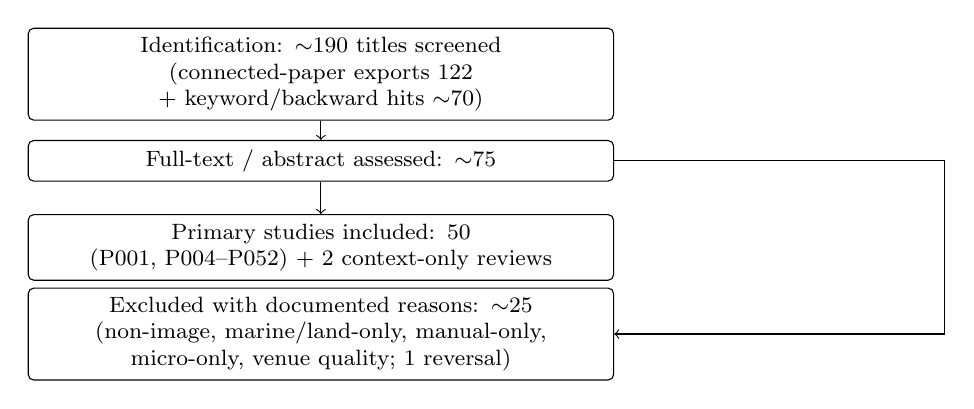
\begin{tikzpicture}[node distance=1.1cm, every node/.style={draw, rounded corners=2pt, text width=7.2cm, align=center, font=\footnotesize}]
\node (id1) {Identification: $\sim$190 titles screened\\(connected-paper exports 122 + keyword/backward hits $\sim$70)};
\node (id2) [below of=id1] {Full-text / abstract assessed: $\sim$75};
\node (inc) [below of=id2] {Primary studies included: 50\\(P001, P004--P052) + 2 context-only reviews};
\node (exc) [below of=inc] {Excluded with documented reasons: $\sim$25\\(non-image, marine/land-only, manual-only,\\micro-only, venue quality; 1 reversal)};
\draw[->] (id1) -- (id2);
\draw[->] (id2) -- (inc);
\draw[->] (id2) -| ([xshift=4.2cm]id2.east) |- (exc);
\end{tikzpicture}
\caption{Selection flow for the review corpus (working counts; single-agent screening with human log review).}
\label{fig:prisma}
\end{figure}


\section{Data Sources and Imaging Platforms}
\label{sec:datasources}

This section answers RQ1: which datasets and imaging platforms underpin riverine waste detection. The base study is UAV-only \cite{Pati2025}; this review expands the frame to satellite, ground, handheld, surface-vehicle, and (absent) underwater sources (Table~\ref{tab:platforms}).

\subsection{Unmanned Aerial Vehicles}
UAVs dominate the corpus, offering millimetre-to-centimetre resolution at the cost of limited coverage, flight permissions, and weather sensitivity. Typical surveys fly 12--90~m yielding 4--30~mm ground sampling distance \cite{Jakovljevic2020,Maharjan2022,Pati2025}. Altitude directly trades against reliability: a multispectral Arno study holds 89.7\% precision at 30~m but collapses to 33.9\% at 80~m under sun glint \cite{Cortesi2022}. UAV RGB is the default modality; multispectral payloads (MAIA-S2 nine-band \cite{Cortesi2022}; MicaSense RedEdge \cite{Iordache2022}) add polymer discrimination at higher operational cost.

\subsection{Satellite Imagery}
Sentinel-2 (10--60~m) enables basin-scale, high-revisit monitoring but is blind to small dispersed items. Multi-river training lets segmentation models transfer across regions \cite{SoleGomez2022}, while single-river pixel classifiers degrade sharply on unseen hydrological conditions \cite{Mohsen2023}. Riverbank-focused indices with vegetation/built-up corrections extend applicability to complex shorelines \cite{Sakti2023}, and an operational three-river pipeline with an open Earth Engine application demonstrates deployment readiness \cite{PerezGarcia2025}. Commercial sub-metre imagery (Pleiades) serves mainly as validation rather than monitoring input \cite{Sakti2023}.

\subsection{Ground, Fixed, and Handheld Cameras}
Bridge- and bank-mounted cameras provide continuous, low-cost observation of fixed reaches and enable flux counting, but cover static fields of view and need power and connectivity \cite{Lieshout2020,Reinhardt2024}. Controlled release experiments on the Rhine reach $\sim$94\% mAP@0.5 with modest data \cite{Reinhardt2024}, while real-stream counting can collapse (6 of 32 items at the counting line) despite near-perfect detection scores \cite{Lee2025}. Handheld and phone imagery lowers the participation barrier for citizen science but introduces angle, scale, and quality inconsistency \cite{JiaFrontiers2023,Tharani2021}; smartphone-collected riparian sets with open releases partially offset this \cite{Pan2024}. Dual fixed-plus-UAV deployments combine persistence with rapid hotspot assessment \cite{FrontEnv2025}.

\subsection{Surface Vehicles and Radar}
Unmanned surface vehicles contribute a novel low-altitude viewpoint plus millimetre-wave radar, with the first inland-waters USV benchmark exposing small-object difficulty across six detectors \cite{Cheng2021}. Unmanned boats and pontoon-mounted cameras extend coverage to inaccessible or infrastructure-adjacent waters \cite{Peng2024,FrontEnv2025}.

\subsection{Hyperspectral and Multispectral Sensing}
Spectral range matters as much as platform: NIR--SWIR signatures separate polymers from water and vegetation where RGB fails. Laboratory-trained classifiers transfer to riverbanks at up to 93.6\% plastic accuracy \cite{Tasseron2022}, and multispectral UAV classification reaches operational precision only at low altitude \cite{Cortesi2022}. A river-systems spectral database now exists as shared infrastructure \cite{Olyaei2024}.

\subsection{Underwater Cameras: An Explicit Gap}
No included study deploys underwater cameras for riverine waste detection; the reference review excludes them by scope, and the closest evidence concerns shallow-water classification degradation \cite{Jakovljevic2020}. Submerged litter is therefore systematically invisible: calibration studies estimate only half of transported litter floats within camera view \cite{Wolf2022}, and field frameworks explicitly cannot yet detect submerged debris \cite{Nunkhaw2025}. This gap is recorded here as found, not filled.

\begin{table}[!t]
\centering
\caption{Imaging platform comparison for riverine waste detection.}
\label{tab:platforms}
\begin{tabular}{lcccc}
\hline
\textbf{Platform} & \textbf{Resolution} & \textbf{Coverage} & \textbf{Cost} & \textbf{Key limitation} \\
\hline
UAV RGB & mm--cm & Reach & Medium & Altitude/permission/weather \\
UAV multispectral & cm & Reach & High & Payload + calibration load \\
Satellite (Sentinel-2) & 10--60~m & Basin/global & Low (open) & Small-item blindness \\
Satellite (commercial) & Sub-metre & Tasked & High & Cost; validation role \\
Fixed bridge/bank & cm & Single reach & Low & Static view; power/network \\
Handheld/phone & mm--cm & Opportunistic & Very low & Inconsistency \\
USV/boat + radar & cm & Reach & Medium & Novelty; sparse methods \\
Underwater & --- & --- & --- & No river studies found \\
\hline
\end{tabular}
\end{table}

\section{Waste Detection Approaches}
\label{sec:approaches}

This section answers RQ2 progressively (classification $\rightarrow$ object detection $\rightarrow$ semantic segmentation $\rightarrow$ instance segmentation) and feeds RQ3. Definitions are kept strict: detection outputs bounding boxes; segmentation outputs pixel masks; instance segmentation outputs masks with instance identity.

\subsection{Image and Pixel Classification}
Classification assigns one label per image, tile, or pixel and suits density estimation, hotspot mapping, and triage. Dual-network designs separate detection from quantification, reaching 83\% and 71\% overall accuracy on airborne river imagery \cite{Wolf2020}. Litter-level classification (none/little/moderate/lots) peaks at 91.7\% with DenseNet121 on canal imagery and generalizes across litter types at fixed geometry \cite{JiaFrontiers2023}. Pixel classifiers on hyperspectral data transfer from laboratory to riverbank at 93.6\% plastic accuracy \cite{Tasseron2022}, while multispectral UAV and satellite classifiers depend critically on altitude and resolution \cite{Cortesi2022,Mohsen2023}. Hotspot mapping with random forests reaches cross-river plastic F1 of 79\% \cite{PerezGarcia2025}. Adjacent infrastructure work classifies screen blockage state rather than items and is treated as deployment evidence only \cite{Vandaele2024}.

\subsection{Object Detection}
Bounding-box detection dominates the corpus (over 30 studies), driven by the YOLO family's speed and maturing accuracy: reported mAP@0.5 spans 65\% on small low-resource sets \cite{Putra2021} to 94\% on controlled bridge releases \cite{Reinhardt2024}, with most river results in the 77--89\% band \cite{Lin2021,Yang2022,Zailan2022,Nunkhaw2024}. Two-stage detectors (Faster R-CNN, RetinaNet, Cascade R-CNN) trade speed for localization, remaining relevant for small-target river work \cite{MPFasterRCNN2024,Cheng2021}. Attention augmentations (feature-map, coordinate, long-range, polarized) consistently add 2--6 percentage points \cite{Lin2021,Yang2022,Peng2024}. Counting overlays (tracking, counter lines, slicing-aided inference) convert detections into flux estimates with mixed reliability \cite{Putra2021,Lee2025,JiaFlux2025}.

\subsection{Semantic Segmentation}
Pixel-level segmentation wins where area, shape, and coverage matter. Fine-tuned DeepLabv3+ outperforms detection counterparts on precision and recall on the same UAV tiles \cite{Pati2025}, and encoder-decoder ResUNet50 maps polymer types at F1 up to 0.92 \cite{Jakovljevic2020}. On satellite imagery, U-Net variants and DeepLabV3+ reach debris IoU around 0.61 on held-out regions but collapse on sediment-shifted rivers \cite{SoleGomez2022}. Segmentation costs more compute and denser annotation, which partly explains its minority share.

\subsection{Instance Segmentation: Emerging}
Only two studies attempt joint masks plus instance identity: custom-trained YOLOv8n-seg beats COCO-pretrained and foundation-model baselines on weathered riparian waste \cite{Pan2024}, and five YOLOv8-based models trained on seven rivers transfer to gauge-camera imagery, with intermediate model sizes beating the largest through avoided overfitting \cite{Kataoka2024}. A key design rule emerges: finer ground sampling favors segmentation while coarser sampling favors detection \cite{Kataoka2024}. The scarcity of instance-level work against its evident value for mass-transport estimation is a central gap (Section~10).

\section{Deep Learning Architectures}
\label{sec:architectures}

This section compares architecture families specifically for riverine waste traits: small targets, occlusion, reflection, vegetation entanglement, and class imbalance.

\subsection{YOLO Family: The Workhorse}
One-stage YOLO detectors appear in over 25 studies, from v2 through v10, because they balance accuracy with deployable speed. Within-family comparisons repeatedly favor lightweight variants for field use: YOLOv5s offers the best accuracy--complexity tradeoff on river UAV imagery while YOLOv4 localizes better at far higher cost \cite{Maharjan2022}; YOLOv8n sustains 0.992 mAP@0.5 on stream footage \cite{Lee2025}; nano-scale models enable Raspberry Pi and RK3588 edge deployment \cite{Sio2022,Yan2025}. Task-specific modifications cluster around attention (feature-map, coordinate, long-range, polarized), improved losses (SIoU, WiseIoU), and feature pyramids (BiFPN, GFPN), each contributing roughly 2--6 points of mAP \cite{Lin2021,Yang2022,Peng2024,Chen2023}. Dark-channel lighting augmentation lifts cross-river mAP@50-95 by 17\% without architectural change \cite{Saddi2024}.

\subsection{Two-Stage and Single-Shot Alternatives}
Faster R-CNN with Inception backbones established the fixed-camera baseline at 68.7\% precision \cite{Lieshout2020} and remains the backbone of self-supervised pipelines \cite{JiaSwAV2024}. RetinaNet variants compete closely with YOLO on canal data \cite{Tharani2021}. SSD persists through lightweight and domain-adaptive niches: teacher-student semi-supervision \cite{Sun2025}, camera-network deployment at 91.1\% \cite{Renfei2023}, and continual unsupervised domain adaptation at 82.2\% and 68.5 FPS \cite{EAAI2023}. Polarized-attention Faster R-CNN variants cut model size fivefold while adding 6.4 points on Yellow River data \cite{MPFasterRCNN2024}.

\subsection{Segmentation Architectures}
Encoder-decoder segmentation (FCN, U-Net family, DeepLabv3+) dominates pixel-level work. Fine-tuned DeepLabv3+ is the strongest single model in the base comparison \cite{Pati2025}; ResUNet50 maps polymer types with F1 up to 0.92 \cite{Jakovljevic2020}; spectral 3D U-Net variants match DeepLabV3+ on satellite debris at IoU 0.61 \cite{SoleGomez2022}. Mask R-CNN serves riverbank quantification pipelines \cite{Trinh2022}, while custom YOLOv8n-seg surpasses both COCO pretraining and foundation-model baselines on weathered litter \cite{Pan2024}.

\subsection{Transformers, Foundation Models, and State-Space Models: Nearly Absent}
No included river study trains a vision transformer as its primary detector; the base paper argues explicitly that CNN inductive biases suit small heterogeneous river datasets, with transformer comparison left as background discussion \cite{Pati2025}. Transformer-assisted segmentation exists only for marine imagery and is excluded by scope. Foundation models appear asymmetrically: as defeated baselines (SAM loses to task-trained YOLOv8n-seg \cite{Pan2024}), as data generators (Stable Diffusion synthetic training sets \cite{Pan2023}), and as inspiration (self-supervised SwAV pretraining toward litter foundation models \cite{JiaSwAV2024}). The first state-space backbone (Changemamba) arrives via semi-supervised UAV detection \cite{Sun2025}. The transformer gap flagged in prior reviews therefore persists into 2025 and is recorded as a first-order research opportunity.

\begin{table}[!t]
\centering
\caption{Architecture families: typical riverine accuracy, cost, and best-fit role.}
\label{tab:archs}
\begin{tabular}{lccc}
\hline
\textbf{Family} & \textbf{Typical mAP} & \textbf{Cost} & \textbf{Best fit} \\
\hline
YOLOv5/v8 nano-small & 77--92\% & Low & Real-time field deployment \\
YOLOv5x/v7-large & 83--94\% & High & Accuracy-first surveys \\
Faster R-CNN/RetinaNet & 65--81\% & High & Small-target precision \\
SSD (+UDA/SSL) & 65--91\% & Low--med & Networks, adaptation \\
DeepLabv3+/U-Net & IoU 0.6--0.87 & High & Area/mass estimation \\
Mask R-CNN/YOLO-seg & mAP 45--59\% & High & Instance quantification \\
Transformers & --- & --- & No river studies found \\
\hline
\end{tabular}
\end{table}

\section{Datasets}
\label{sec:datasets}

This section answers the dataset half of RQ1 through a master comparison (Table~\ref{tab:datasets}), including the base paper's novel sets.

\subsection{Scale and Annotation Landscape}
Dataset sizes span two orders of magnitude: 340-image low-resource sets \cite{Putra2021} to 16,000-image canal collections \cite{Qiao2022}, 14,925-image hyacinth surveys \cite{Saigon2025}, and 2,000-image multimodal benchmarks with 20,000 unlabeled tracking frames \cite{Cheng2021}. Annotation follows task: VOC boxes for detection, COCO polygons for instance work, pixel masks for segmentation. The largest open resources are the canal TUD-GV set (9,473 images \cite{JiaFrontiers2023}), the riparian HRB-WD set with released weights \cite{Pan2024}, the canal water-channel set (13,500 images, 48,450 objects \cite{Tharani2021}), and the USV-view FloW benchmark \cite{Cheng2021}. The base paper contributes 764 dual-annotated UAV tiles (detection plus segmentation) from two Nepali rivers via public repository \cite{Pati2025}, and the Laos--Thailand study adds 500 tiles per site at 2~m ground footprints \cite{Maharjan2022}.

\subsection{Category and Condition Coverage}
Most sets collapse waste into one ``waste'' or ``plastic'' class, which simplifies annotation but discards polymer information; exceptions separate bottles, bags, foam, organics, and vegetation \cite{Lin2021,Nunkhaw2024,Tharani2021}. Weathered, submerged, transparent, and entangled items are systematically under-annotated: dataset authors explicitly exclude micro-particles and leaves \cite{Tharani2021}, and field frameworks report transparency and hyacinth entrapment as dominant miss drivers \cite{JiaFlux2025,Nunkhaw2025}. Vegetation-heavy tropical sets (69k plastics against 57k hyacinths \cite{Saigon2025}) are the exception that proves the rule.

\subsection{Geographic and Modal Diversity Gaps}
Collection concentrates in Europe, East and South Asia; African and South American river datasets are essentially absent from the deep-learning corpus despite field studies confirming heavy pollution there \cite{Atuhaire2025}. No underwater river-waste dataset exists. Radar appears once as a modality \cite{Cheng2021}; synthetic data appears once as training source \cite{Pan2023}; self-supervised pools ($\sim$100k unlabeled images \cite{JiaSwAV2024}) point toward foundation-scale collection as the structural fix the field keeps requesting.

\begin{table}[!t]
\centering
\caption{Master dataset comparison (selected; TBD = unreported).}
\label{tab:datasets}
\begin{tabular}{lccccc}
\hline
\textbf{Dataset} & \textbf{Images} & \textbf{Annot.} & \textbf{Region} & \textbf{Resol.} & \textbf{Access} \\
\hline
P001 Bagmati/Bishnumati & 764 & Box+mask & Nepal & 256px UAV & Public \\
P004 Balkana/Crna Rijeka & 328/434/1846 & Pixel & Bosnia & 256px UAV & TBD \\
P006 HMH/TT & 500+500 & Box & Laos/Thai & 256px UAV & TBD \\
P008 TUD-GV & 9,473 & Level & Neth. canal & 1080p & Public \\
P012 Lahore canals & 13,500 & Box+mask & Pakistan & TBD & Partial \\
P017 HRB-WD & TBD & Mask & Japan & Phone 48MP & Public+weights \\
P027 7-river + WLGCAM & 7,356+3,802 & Box+mask & Japan & Fixed cam & TBD \\
P031 Korea stream & 4,162+1,005 & Box & Korea & Video & TBD \\
P036 Citarum/Motagua/Odaw & TBD & Pixel & ID/GT/GH & S2 10m & Partial (app) \\
P038 SSL pool & $\sim$100k unl. & Box (1.8k) & NL/ID/VN & Fixed cam & Public \\
P042 Saigon & $\sim$15k & Box & Vietnam & UAV+fixed & TBD \\
P048 FloW/FloW-RI & 2,000+videos & Box+radar & TBD inland & USV & Likely public \\
\hline
\end{tabular}
\end{table}

\section{Training Strategies and Generalization}
\label{sec:training}

\subsection{From Scratch, Fine-Tuning, and Frozen Layers (RQ4)}
The base comparison establishes task-dependent optima: full-model fine-tuning wins for segmentation while frozen backbones win for detection, both substantially above training from scratch \cite{Pati2025}. The predecessor study concurs with a nuance: fine-tuning beats frozen-only marginally (3\% vs.\ 1\% gains) but both dwarf scratch training, with the largest scratch-to-transfer jump on the weakest architecture (YOLOv3-spp 0.59 to 0.81 mAP) \cite{Maharjan2022}. For classification, fine-tuning all layers beats classifier-only tuning, and simple flipping is the most cost-effective augmentation \cite{JiaFrontiers2023}. Optimizer discipline matters at the margin: SGD at low learning rates with patience-based early stopping outperforms Adam configurations \cite{WCSE2024}.

\subsection{Cross-River and Cross-Site Transfer (RQ5)}
Geographically proximate transfer works: cross-river fine-tuning reaches mIoU 0.849/0.841 \cite{Pati2025} and cross-country canal-to-river transfer adds up to 3 points \cite{Maharjan2022}. Cross-continent deployment succeeds when paired with lighting augmentation, gaining 17\% mAP@50-95 \cite{Saddi2024}. Fixed-camera models hold $\sim$50\% average precision on similar new sites without retraining, and 50 new-location objects lift different-condition precision from 20\% to 42\% \cite{Lieshout2020}. Seven-river training transfers to novel gauge-camera imagery \cite{Kataoka2024}, canal-trained classifiers hold on unseen litter at fixed geometry \cite{JiaFrontiers2023}, and test sets drawn from held-out sites validate urban-canal detectors \cite{Tharani2021}. Failures bound the claims: sediment-shifted rivers collapse segmentation to 0.02 IoU \cite{SoleGomez2022}, and land-trained classifiers do not transfer directly to water \cite{Iordache2022}.

\subsection{Data-Centric and Self-Supervised Strategies (RQ4)}
Three families reduce annotation dependence. First, preprocessing-as-transfer adapts laboratory-trained models to real canals without retraining (mAP 0.74 to 0.85) \cite{Nunkhaw2025}, and tiling plus blurring rescues small and vegetated targets \cite{FrontEnv2025}. Second, self- and semi-supervision: teacher-student training lifts mAP 75.1\% to 77.7\% with unlabeled data \cite{Sun2025}; SwAV pretraining on $\sim$100k river images adds up to 12.7\% zero-shot average precision over ImageNet transfer \cite{JiaSwAV2024}; SSL plus slicing-aided inference adds 45 small items and doubles supervised flux estimates \cite{JiaFlux2025}. Third, synthetic and web supplementation: diffusion-generated imagery trains competitive detectors on simple backgrounds \cite{Pan2023}, while web data helps only when ground-sampling matched and combined with site data \cite{Pan2022}. Continual unsupervised domain adaptation across lighting and weather adds up to 13.4 points over prior adaptive detectors \cite{EAAI2023}.

\section{Evaluation: Metrics, Speed, and Cost}
\label{sec:evaluation}

Metrics are reported strictly within task scope: detection mAP, segmentation IoU, classification accuracy, and counting reliability are not pooled.

\subsection{Detection and Segmentation Metrics}
Object-detection mAP@0.5 spans 65\% on tiny low-resource sets to 94\% on controlled releases, clustering at 77--89\% for river work. Small-target metrics reveal a crisis averages conceal: small-object average precision sits at 2.7--5.2\% even in strong pipelines \cite{Tharani2021}, motivating attention heads, slicing inference, and tiling \cite{Lin2021,JiaFlux2025,FrontEnv2025}. Segmentation mIoU ranges from $\sim$0.5 on satellite debris to 0.87 on UAV tiles \cite{SoleGomez2022,Pati2025}, with polymer-level F1 up to 0.92 \cite{Jakovljevic2020} and debris IoU 0.61 on held-out regions \cite{SoleGomez2022}. Classification accuracy spans 83--95\% across airborne, canal, hyperspectral, and multispectral settings \cite{Wolf2020,JiaFrontiers2023,Tasseron2022,Cortesi2022}.

\subsection{Speed and Computational Cost}
Where reported, efficiency favors nano-scale one-stage models: 3.1~ms per frame at 8.3M parameters \cite{Liu2025}, 30.5~ms on edge hardware \cite{Yan2025}, $\sim$100~ms TensorRT-accelerated streams \cite{FrontEnv2025}, and tenfold compression via separable convolutions at modest accuracy cost \cite{Tharani2021}. Most studies omit speed and cost entirely; absence is stated rather than imputed.

\subsection{From Detection Scores to Trustworthy Counts}
High detection scores do not imply reliable quantification: a 0.992 mAP@0.5 model counts 6 of 32 debris items on unseen video \cite{Lee2025}; dense aggregations defeat tracking-based counting \cite{FrontEnv2025}; and the best flux framework underestimates human measurements three- to fourfold on transparent and entrapped items \cite{JiaFlux2025}. inflated overall accuracy under class imbalance (water majority) further cautions against headline metrics \cite{Mohsen2023}. Evaluation for riverine waste must therefore report counting-conditioned metrics alongside detection scores.

\section{Challenges and Research Gaps}
\label{sec:challenges}

\subsection{Small, Transparent, and Submerged Targets}
Small-object average precision below 6\% persists even in strong pipelines \cite{Tharani2021}, glass and transparent plastics score lowest across studies \cite{Nunkhaw2024}, and transparency plus hyacinth entrapment drive three- to fourfold flux underestimation \cite{JiaFlux2025}. Calibration evidence suggests only half of transported litter floats within camera view \cite{Wolf2022}, and current field frameworks explicitly cannot detect submerged debris \cite{Nunkhaw2025}. The gap is therefore measurement-complete, not merely algorithmic.

\subsection{Vegetation Entanglement and Water Conditions}
Water hyacinths carry 73\% of floating plastics at 197-fold concentration factors \cite{Saigon2025}, turning vegetation from background noise into the primary transport vector. Sun glint collapses multispectral precision from 89.7\% to 33.9\% with altitude \cite{Cortesi2022}; reflections, shadows, turbidity, and rainfall defeat detectors trained in narrow conditions \cite{Lin2021,Tharani2021,Putra2021,Lee2025}. Sediment regime shifts alone can zero out transferred segmentation \cite{SoleGomez2022}.

\subsection{Data Scarcity, Annotation Cost, and Standardization}
Labeling is repeatedly the binding constraint \cite{Jia2023,JiaFrontiers2023,Lin2021}. Internal inconsistencies in published metrics (see contradiction records C004--C005) and headline-accuracy inflation under class imbalance \cite{Mohsen2023} show the field also lacks reporting discipline, a problem harmonization literature independently diagnoses \cite{Hurley2023}. Flux and hotspot quantification methods remain rare and incomparable \cite{Lieshout2020,JiaFlux2025}.

\subsection{Geographic, Modal, and Architectural Imbalances}
Deep-learning river datasets cluster in Europe and Asia while African and South American rivers contribute field evidence but almost no training data \cite{Atuhaire2025}. No underwater river-waste dataset or study exists. Transformers have no river-waste primary study despite their dominance elsewhere, and foundation models appear only as baselines, data generators, or inspiration rather than deployed solutions.

\section{Future Research Directions}
\label{sec:future}

Each direction below answers a gap from Section~\ref{sec:challenges} and names an actionable first step.

\subsection{Measure What Cameras Miss}
Develop submerged-capable river sensing (low-light architectures, polarization, depth cues) and report floating versus total-transport fractions with net-calibrated protocols, following the bridge-plus-net template \cite{Wolf2022}. Benchmarks should include transparency and entrapment stress splits rather than clean-water test sets \cite{JiaFlux2025}.

\subsection{Model Vegetation Jointly}
Treat hyacinth and debris as a joint detection problem with entrapment-aware labels, and empirically test the hyacinth-as-satellite-proxy and joint-removal hypotheses that current work only proposes \cite{Saigon2025}. Preprocessing that suppresses vegetative noise (tiling, blurring, background removal) should become standard reporting \cite{FrontEnv2025,Nunkhaw2025}.

\subsection{Build for Adverse Conditions}
 Adopt illumination-robust training (dark-channel and test-time lighting sweeps \cite{Saddi2024}), weather-adaptive detectors \cite{EAAI2023}, and multispectral or hyperspectral sensing where RGB saturates \cite{Cortesi2022,Tasseron2022}. Publish per-condition metric breakdowns instead of single headline scores.

\subsection{Scale Data Without Scaling Cost}
Prioritize open datasets with released weights \cite{JiaFrontiers2023,Pan2024,JiaFlux2025,Cheng2021}, semi- and self-supervised pipelines that exploit unlabeled river footage \cite{Sun2025,JiaSwAV2024}, synthetic supplementation for well-scoped settings \cite{Pan2023}, and citizen-science collection with standardized protocols \cite{Lieshout2020,Cook2021,RiverWatch2024}. Target Global-South rivers to correct the geographic imbalance \cite{Atuhaire2025}.

\subsection{Close the Architecture and Evaluation Gaps}
Run the first controlled transformer-versus-CNN comparisons on fixed river benchmarks; extend state-space and edge-efficient backbones to deployment studies \cite{Sun2025,Yan2025}; require counting-conditioned metrics (tracking F1, flux error versus human counts) alongside detection scores \cite{Lee2025,JiaFlux2025}; and converge on harmonized reporting discipline \cite{Hurley2023}.

\section{Conclusion}
\label{sec:conclusion}

This review asked how well deep-learning-based waste detection generalizes beyond its training environment, synthesizing 50 studies across platforms (Section~\ref{sec:datasources}), approaches (Section~\ref{sec:approaches}), architectures (Section~\ref{sec:architectures}), datasets (Section~\ref{sec:datasets}), training strategies (Section~\ref{sec:training}), and evaluation practice (Section~\ref{sec:evaluation}). Three findings stand out. First, transfer works within bounds: proximate rivers, similar sites, and matched spectra transfer reliably, while sediment shifts, land-to-water jumps, and marine-to-river leaps do not. Second, the field is solving annotation scarcity faster than it is solving measurement completeness: open datasets, self-supervision, synthetic supplementation, and adaptation recover data efficiency, yet submerged, transparent, and entangled litter still defeats quantification. Third, evaluation lags capability: detection scores systematically overstate counting and flux reliability.

The review itself is limited by seed-anchored (not exhaustive) collection, single-agent screening, English-only sources, a 2019--2025 window, and provisional rows quarantined from strong claims. On the base study \cite{Pati2025}, this review supports its cross-river transfer finding across many independent replications while qualifying its training-strategy finding as architecture- and task-dependent. Its contribution is the first generalization-centered synthesis of the field with explicit evidence grading, giving practitioners a transferability map and researchers a gap inventory with actionable next steps.


\bibliographystyle{IEEEtran}
\bibliography{../sections/references}

\EOD
\end{document}
